\chapter{Revue de littérature}
\label{ch:litterature}

\section{Historique et concepts de la RA}
\label{sec:litterature_ar}

\cite{Sutherland1968} conçoit le premier visiocasque de RA \reffigureETSp{Sutherland1968.jpg} : ce prototype permet déjà de visualiser du contenu 3D affiché dans l'espace réel de l'utilisateur, donnant l'illusion que le contenu virtuel fait réellement partie de la pièce. Par la suite, la recherche académique en RA se développe lentement : les applications développées sont surtout à visées militaires et gouvernementales \citep{VanKrevelen2010}. Il faut alors attendre les années 1990, avec la miniaturisation des PCs, pour que le domaine de recherche s'établisse enfin. Plusieurs conférences dédiées à la RA sont notamment créées, fusionnées aujourd'hui sous le nom de International Symposium on Mixed and Augmented Reality (ISMAR), une conférence d'importance pour la recherche et l'industrie en RA \citep{Azuma2001}.

\figureETS[0.6]{Sutherland1968.jpg}{
  Photos du visiocasque de RA de Sutherland.\\
  Tiré de \cite{Sutherland1968}.
}

\cite{Milgram1994} donne un premier cadre théorique au domaine, en proposant une échelle ordonnée nommée \texten{Reality-Virtuality Continuum} \reffigureETSp{Milgram1994}. \citeauthor{Milgram1994} y oppose deux extrèmes : les environnements réels et les environnements virtuels. Les IHMs habituelles sur ordinateurs et téléphones, ou encore \texten{graphical user interface} (GUI), font partie de la première catégorie, tandis qu'un visiocasque de RV, qui immerge totalement son utilisateur dans un monde virtuel, de la seconde. Entre ces deux extrêmes, les environnements de Réalité Mixte (RM), comme la RA, vont mélanger éléments réels et virtuels. La force de cette représentation est qu'il n'existe pas de catégories séparées entre réel, RA et RV mais que la RA peut se trouver d'un extrème à un autre le long de cette échelle.

Le second enseignement de l'échelle de \citeauthor{Milgram1994} est que RA et RV sont techniquement très proches : les dispositifs de localisation, d'affichage et de géneration de contenu sont les mêmes \citep{Billinghurst2015}. Cependant, ces deux technologies n'ont pas les mêmes attentes. En effet, pour que l'immersion en RV fonctionne, il est nécessaire d'avoir un large champ de vision ; par exemple, le champ de vision du visiocasque de RV HTC Vive est de \SI{100x113}{\degree} (horizontalement $\times$ verticalement) pour les deux yeux \citep{Kreylos2016}, ce qui est proche du champ de vision humain qui est de \SI{200x135}{\degree} pour les deux yeux (\url{https://biology.stackexchange.com/a/28140}). La RA va en revanche demander tout d'abord une très grande précision et rapidité dans la localisation de l'utilisateur et des objets à augmenter pour donner le sentiment de « présence » du virtuel dans l'environnement réel.

\figureLayoutETS{Milgram1994}{%
  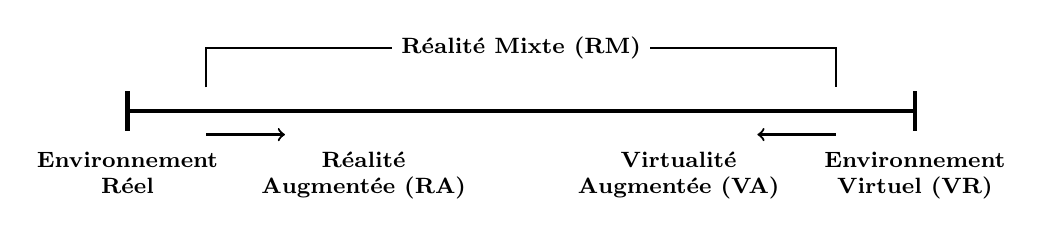
\begin{tikzpicture}[font=\footnotesize\bfseries]
    \tikzstyle{label}=[below, align=center, text depth=.25ex]
    
    \draw[ultra thick] (0,0) -- (10,0);
    \draw[ultra thick] (0,-0.25) -- (0,0.25);
    \draw[ultra thick] (10,-0.25) -- (10,0.25);

    \draw[thick, ->] (1,-0.3) -- (2,-0.3);
    \draw[thick, <-] (8,-0.3) -- (9,-0.3);

    \draw (0,-0.4) node[label] {Environnement\\Réel};
    \draw (3,-0.4) node[label] {Réalité\\Augmentée (RA)};
    \draw (7,-0.4) node[label] {Virtualité\\Augmentée (VA)};
    \draw (10,-0.4) node[label] {Environnement\\Virtuel (VR)};

    \draw[thick] (1,0.3) -- (1,0.8) -- (9,0.8) -- (9,0.3);

    \draw (5,0.8) node[fill=white] {Réalité Mixte (RM)};
  \end{tikzpicture}%
}{
  L'échelle du \texten{Reality-Virtuality Continuum} de Milgram.\\
  Adapté de \cite[p. 3]{Milgram1994}.
}

\cite{Rekimoto1995} apportent un second cadre théorique à la RA \reffigureETSp{Rekimoto1995.png}. Ils montrent que les GUI sont coupées des interactions avec l'environnement réel, tandis que la RV isole l'utilisateur dans des IHMs totalement virtuelles. Deux approches à ces extrèmes sont la RA et l'informatique ubiquitaire (en anglais: \texten{ubiquitous computing}) : cette dernière permet à l'utilisateur d'interagir avec des ordinateur intégrés dans l'environnement réel, par exemple avec téléphones intelligents et des objets connectés, tandis que la RA fusionne réel et virtuel en un seul environnement pour l'utilisateur. Ainsi, avec une IHM bien faite, la RA s'intègre naturellement à l'environnement réel et devient invisible à l'utilisation.

\figureETS{Rekimoto1995.png}{
  Comparaison de quatre styles d'IHMs : (a) les GUI, coupées de l'environnement réel, (b) les IHMs en VR, isolant l'utilisateur dans un environnement virtuel, (c) l'informatique ubiquitaire, faite d'ordinateurs faisant partie intégrante de l'environnement réel et (d) les IHMs en RA faisant interface entre l'utilisateur et l'environnement réel.\\
  Tiré de \cite{Rekimoto1995}.
}

Une première définition formelle de la RA est par la suite proposée par \cite{Azuma1997} dans le premier état de l'art du domaine. Ainsi, la RA :
\begin{enumerate}
  \item combine des éléments réels et virtuels ;
  \item est interactive en temps réel ;
  \item aligne les éléments virtuels avec les éléments réels.
\end{enumerate}
Ce sont les trois conditions techniques à respecter en RA et qui vont permettre le \emph{sentiment de la présence du virtuel} dans l'environnement réel, c'est-à-dire à notre cerveau de voir virtuel et réel comme un seul et même environnement. Cette définition a le mérite d'être assez générale pour s'appliquer tout autant à la RA visuelle, qu'au RA auditives ou haptiques.

\figureETS{Bimber2005.jpg}{
  Les différents dispositifs d'affichages en RA.\\
  Tiré de \citet[p. 72]{Bimber2005}.
}

Enfin, \cite{Buxton1998} repris par \cite{Bimber2005} catégorisent les différents dispositifs d'affichage en RA \reffigureETSp{Bimber2005.jpg}. On retient essentiellement (nous excluons volontairement les projecteurs) :
\begin{itemize}
  \item Le \texten{cave automatic virtual environnement} (CAVE) : c'est un environnment immersif sous forme de cube de \SI{3}{\m^{3}}, chaque face comportant un écran \reffigureETSp{CAVE.jpg}. Les capteurs portés par l'utilisateur permettent au CAVE de suivre son mouvement et ainsi recalculer son champ de vision en temps réel. C'est un dispositif coûteux et encombrant, mais très utile pour prototyper des concepts.
  \item Les affichages fixes : la RA est affichée à travers un écran fixé dans l'environnement \reffigureETSp{Lee2013.jpg}. Ils sont utiles pour des démonstrations pour plusieurs personnes à la fois.
  \item Les appareils mobiles : identique à un affichage fixe mais l'écran est tenu en main, comme une \emph{fenêtre sur le contenu} en RA \reffigureETSp{MobileAR.jpg}. Ils sont populaires mais limités en taille et en puissance \citep{Huang2013}.
  \item Les \texten{head-mounted display} (HMD) ou visiocasques en français : ils sont portés sur la tête et projetent les images virtuelles directement aux yeux de l'utilisateur. Ils ont l'avantage de laisser les mains libres. On distingue deux technologies :
  \begin{itemize}
    \item Les visiocasques vidéo : des caméras placées devant le casque filment l'environnement de l'utilisateur, les images capturées sont ensuite combinées avec le contenu virtuel puis affichées sur un écran \reffigureETSp{ARRift.jpg}.
    \item Les visiocasques optique : le contenu virtuel est projeté sur un écran transparent par un système de mirroirs \reffigureETSp{HoloLens.jpg}.
  \end{itemize}
  \item Les lentilles : elles sont identiques aux visiocasques mais posées directement sur les yeux. Peu utilisées, elles sont encore au stade de prototype mais une fois maîtrisées, elles pourront être à l'avenir le dispotif de RA idéal \citep{VanKrevelen2010}.
\end{itemize}

\figureETS[0.7]{CAVE.jpg}{
  Un CAVE : un cube immersif d'écrans à taille humaine réagissant aux déplacement de l'utilisateur. Ici, l'utilisateur tape la main de son propre hologramme.\\
  Tiré de \cite{Kreylos2012}.
}

\figureETS{Lee2013.jpg}{
  Photos de SpaceTop : l'utilisateur peut interagir avec du contenu 3D à travers un écran transparent.\\
  Tiré de \cite{Lee2013}.
}

\figureETS[0.5]{MobileAR.jpg}{
  Une application sur tablette affichant un tableau de musée en RA.\\
  Tiré de \cite{KWC2012}.
}

Tout ces dispositifs ont été explorés dans la recherche, mais ce sont essentiellement des prototypes sur appareils mobiles qui ont été développés : en effet, à partir des années 2000, les téléphones intelligents ont eu des caméras intégrées d'une qualité suffisante, tous les capteurs nécessaire et assez de puissance de calcul pour rendre la RA possible \citep{Huang2013}. Cependant, avec l'arrivée du Microsoft HoloLens en 2016 les visiocasques vont pouvoir être à leur tour plus utilisés dans des recherches en RA.

Dans leur état de l'art \cite{Azuma2001} identifient les trois obstables à dépasser pour que la RA puisse être utilisable par le grand public : (1) les limites techniques, (2) les limites des IHMs et (3) les problème d'acception sociale. Cependant, si quelques concepts et cadres théoriques pour la RA existent depuis plusieurs années, la recherche s'est malgré tout majoritairement consacrée à dépasser les limites techniques de la RA, comme le souligne \cite{Zhou2008}, \cite{VanKrevelen2010} et \cite{Billinghurst2015}, dans leurs états de l'art respectifs. Ils indiquent également que trop peu de travaux ont été consacrés aux IHM et à l'expérience utilisateur en RA : \textquote{there is a need to develop interface metaphors and interaction techniques specific to [augmented reality]} \citep{Billinghurst2015}.


\section{Conception et évaluation d'IHMs de RA}
\label{sec:litterature_ar_hci}

\subsection{IHMs en RA}
\label{subsec:litterature_ar_hci_presentation}
Une IHM consistue la principale interface, l'intermédiaire, avec laquelle un utilisateur va interagir avec un ordinateur. Sa bonne conception est donc nécessaire pour rendre accesible et efficace le travail sur une machine. Son rôle est simple : comme le montre la \reffigureETS{Billinghurst2005}, il s'agit de lier des entrées utilisateurs issues de capteurs physiques (souris, écran tactile, images d'une caméra) à des actions sur l'ordinateur (affichage, son, commande) via une technique d'interaction, c'est-à-dire une méthode pour faire cette liaison \citep{Billinghurst2005}. La technique d'interaction est donc une métaphore qui permet à l'utilisateur d'associer ses actions avec des résultats sur l'ordinateur : par exemple, bouger un curseur avec sa souris, déplacer une carte en balayant de son doigt l'écran tactile ou encore activer des éléments en les \textquote{touchant} avec une main virtuelle. Il existe de nombreux dispositifs d'entrée, de sortie et de techniques d'interaction, le défi étant de : \textquote{\texten{combine these together in a way that is most appropriate to the desired task, facilitates ease of use and learning and provides a high level of user performance and satisfaction}} \citep{Billinghurst2005}.

\figureLayoutETS{Billinghurst2005}{%
  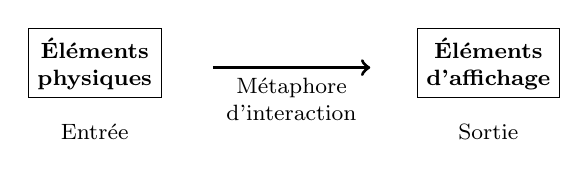
\begin{tikzpicture}[font=\footnotesize]
    \tikzstyle{label}=[below, align=center, text depth=.25ex]
    
    \draw (0,0) node[label, draw]{\textbf{Éléments}\\\textbf{physiques}};
    \draw (5,0) node[label, draw]{\textbf{Éléments}\\\textbf{d'affichage}};

    \draw[->, very thick] (1.5,-0.5) -- (3.5,-0.5)
      node[label, pos=0.5, below]{Métaphore\\d'interaction};

    \draw (0,-1.1) node[label]{Entrée};
    \draw (5,-1.1) node[label]{Sortie};
  \end{tikzpicture}%
}{
  Principe d'une IHM : une technique interaction lie des entrées utilisateur, via un capteur physique, à un résultat affiché sur l'ordinateur.\\
  Adapté de \cite[p. 1]{Billinghurst2005}.
}

La RA représente donc un excellent média car l'écart entre les éléments physiques et virtuels y est très réduit. Cela permettrait, d'une part, de fondre la présence de l'ordinateur dans l'environnement de l'utilisateur et ne plus la restreindre sur un écran d'ordinateur ou d'un téléphone intelligent. Une bonne IHM de RA permettrait alors, d'autre part, de manipuler naturellement et efficacement du contenu virtuel en 3D avec des techniques d'interactions basées sur des objets physiques, des commandes vocales ou des gestes utilisés au quotidien \citep{Billinghurst2005}.

C'est en réalité un des but visé par la recherche en IHM : \cite{VanDam1997} et \cite{Jacob2008} rapellent que les interactions avec les ordinateurs sont allées en plusieurs génerations visant à chaque fois une utilisation plus simple, plus directe et plus proche des actions quotidiennes. Les ordinateurs s'utilisaient par des cartes de commandes et des résultats imprimés (avant 1960), puis avec une ligne de commandes via des terminaux avec clavier (jusque dans les années 1980), enfin par des interfaces graphiques \reffigureETSp{Jacob2008.jpg}. Cette troisième génération d'IHM suit le paradigme WIMP : un ensemble de fenêtres (\texten{windows}), icônes (\texten{icons}) et menus (\texten{menus}) accessibles par un appareil de pointage (\texten{pointing device}), comme une souris. Ces IHMs sont excellentes pour des applications graphiques en 2D, mais limitées, entre autres, pour celles en 3D. \cite{VanDam1997} appella alors à développer une nouvelle génération d'IHMs \textquote{post-WIMP}, contenant des techniques d'interactions non dépendantes de fenêtre, icônes ou de menu en 2D. L'objectif étant de diversifier les types d'IHM pour proposer le plus adapté selon les besoins de l'utilisateur.

\figureETS[0.5]{Jacob2008.jpg}{
  Illustrations des deuxième et troisième générations d'IHM, en ligne de commande puis par interfaces graphiques WIMP, ainsi que les nombreux types émergeants d'IHMs \textquote{post-WIMP}. Toutes sont complémentaires, chacune étant adapté à des usages spécifiques qu'étudie la recherche sur les IHMs.\\
  Tiré de \cite{Jacob2008}.
}

Si de nombreuses IHMs \textquote{post-WIMP} ont par la suite été développées, comme celles désormais bien connues des téléphones intelligents à écrans tactiles \cite{Jacob2008}, aucun paradigme pour la RA n'est encore établi \citep{VanKrevelen2010}. \cite{Billinghurst2005} décrit que ce processus se déroule en quatre étapes : (1) développement de prototypes, (2) adoption de techniques d'interactions d'autres types IHMs, (3) développement de métaphores spécifiques au média, (4) développement de paradigmes de conception d'IHM pour le média. De nombreuses techniques d'interactions ont été développées en RA, mais un effort de conception est encore nécessaire pour atteindre la quatrième étape : \cite{Billinghurst2015}

Billinghurst2015, p. 165 : il y a maintenant plein de méthodes d'interactions mais encore besoin d'effort de conception
There have been a number of AR interface types developed since the 1960’s, including:\\
1) Information Browsers: Interfaces for showing AR information on the real world\\
2) 3D User Interfaces: Using 3D interaction techniques to manipulate content in space\\
3) Tangible User Interfaces: Using real objects to interact with AR virtual content\\
4) Natural User Interfaces: Using natural body input such as free hand gestures\\
5) Multimodal Interfaces: Using combined speech and gesture input\\

Discuter des IHM sur mobile pendant les années 2000 et 2010 (information Browsers dans la classification de Billinghurst2015)

Billinghurst2015, p.179 : par contre clairement besoin de recherche dans les interfaces\\
+ étapes construction d'IHM pour la RA (le WIMP est passé par là) :\\
1) Prototype Demonstration\\
2) Adoption of Interaction techniques from other interface metaphors\\
3) Development of new interface metaphors appropriate to the medium\\
4) Development of formal theoretical models for modelling user in teractions\\
La plupart des IHM en RA ne vont pas au dela des étapes 1 et 2. Vs VR qui en est à l'étape 3 (Go-Go, controlleurs, gaze)\\
MacIntyre points out that AR design is driven by the need to define and fuse the relationship between entities in the physical world and virtual world [MacIntyre, 2002]

there are three components that must be designed in an AR application (see Figure 8.1): (1) the real physical objects, (2) the virtual elements to be displayed, and (3) the interaction metaphor that links the real and virtual elements together.\\
1 et 2 : affordances visuelles pour faire comprendre comment peuvent être manipulés. La technique d'interaction lie 1 et 2

\subsection{Interactions en 3D}
\label{subsec:litterature_ar_hci_interactions}
Si les interactions sur des surfaces tactiles comme les téléphones intelligents sont bien maîtrisées, les interactions dans les environnements en 3D sont moins connues.

Berard2009 : c'est quoi une technique d'interaction : « « Interaction is not defined by an input device alone, but by the combination of a device and an interaction technique. In the example of 3D object rotation, the mouse is typically used with the virtual sphere technique while a free-space device is used with a direct mapping (either absolute or relative) Thus, each device must be matched with its most suitable interaction technique in making performance comparisons, rather than choosing a single interaction technique for all devices. » »

Bowman2004 : summarizes various types of 3D interactions into three categories: (1) navigation, (2) selection, and (3)
manipulation

Argelaguet2013 : pb des interactions 3D, sélection tâche + métaphores main et gaze, subjectivité vs performance, design technique, taxonomie technique,  (voir cahier gris)\\
Métaphore main virtuelle : cependant, cette technique amène un autre problème quand elle est utilisée en RA. En effet, en RA, le contenu virtuel est « imprimé par dessus » le contenu réel et peut donc masquer le contenu réel. Par exemple, je peux vouloir toucher un objet 3D en l'air avec ma main, mais cette dernière sera toujours masqué par l'objet même si ma main semble en avant de l'objet. Dès lors, il faut utiliser une technique d'occlusion, c'est-à-dire masquer l'objet 3D quand un objet réel, comme la main de l'utilisateur, se trouve devant \reffigureETSp{Piumsomboon2014_1}.

\figureLayoutETS{Argelaguet2013}{%
  \subfigureETS[0.25]{Argelaguet2013_1.jpg}{Main virtuelle}%
  \figurehspace%
  \subfigureETS[0.25]{Argelaguet2013_2.jpg}{Pointeur virtuel}%
}{
  Différentes techniques de sélection.\\
  Adapté de \cite{Argelaguet2013}.
}

Bowman2001 : Principal problème est qu'il n'y a aucun retour tactile « touching a menu item floating in space is much more difficult than selecting a menu item on the desktop, not only because the task has become 3-D, but also because the impor- tant constraint of the physical desk on which the mouse rest is missing. »\\
Chan2010 - Touching the void : mid air touch in intangible displays. Naturle car simplifie la manip d'objet : le display et l'interactions sont combinés (de la même manière qu'on manipule des objets réels). Expérience d'acquisition d'objets : les personnes évaluent mal la profondeur de leur doigt (donc quand elles ont touché la cible), car pb double vision : vise le doigt et donc cible est floue. Conclusion : il faut utiliser des retours visuels pour guider l'utilisateur. Deux types de feedbacks : continu pour situer sa main, discret pour confirmer une action.

Berard2009 : input en 2D est plus performant

Piumsomboon2013 : fait une taxonomie des gestes mid-air pour l'AR, sur le modèle de Wobbrock2009 -> à évaluer sur des interfaces

\cite{Piumsomboon2014} ont comparé différentes techniques de sélection et de manipulation d'objets 3D avec un visiocasque de RA : des interactions avec la main et des commandes vocales \reffigureETSp{Piumsomboon2014_2}. Une des première leçon de leur travail est sur l'occlusion des mains avec le contenu virtuel : dans une étude pilote, ils ont remarqué que les utilisateurs n'avaient pas de préférence entre l'occlusion de la main avec le contenu 3D ou ajouter de la transparence à ce contenu virtuel \reffigureETSp{Piumsomboon2014_1}. L'occlusion de la main virtuelle étant un problème difficile à résoudre et lourd en calcul, la transparence sur le contenu virtuel en RA est une solution simple à mettre en oeuvre, comme a pu le faire \cite{Lee2013} avec SpaceTop.

\figureLayoutETS{Piumsomboon2014_1}{%
  \subfigureETS[0.2]{Piumsomboon2014_1.jpg}{Main virtuelle faisant occlusion avec le contenu 3D.}%
  \figurehspace%
  \subfigureETS[0.2]{Piumsomboon2014_2.jpg}{Contenu 3D transparent laissant la main virtuelle visible.}%
}{
  Différentes techniques d'occlusion de la main.\\
  Tiré de \cite{Piumsomboon2014}.
}

Dans une seconde expérience, \citeauthor{Piumsomboon2014} ont également trouvé que les participants préféraient utiliser et étaient plus performants avec les interactions manuelles plutôt que vocales sur les tâches de manipulation et de rotation d'objets. Les participants ont par contre préféré les commandes vocales pour modifier la taille des objets 3D, sans qu'il n'y ait de différence de performance avec les interactions manuelles. Les auteurs suggèrent donc de combiner les deux types d'interactions dans les IHMs de RA. Une limite du travail de \citeauthor{Piumsomboon2014} cependant est de n'avoir pas étudié de techniques de navigation. De plus, les interactions étaient conçues et étudiées pour manipuler des objets en 3D : une IHM de RA peut demander d'interagir avec des données plus abstraites, comme le sont nos interfaces graphiques sur ordinateur et téléphone actuellement. Les résultats de cette étude sont donc intéressant pour des métier manipulant de la 3D, mais il serait intéressant de savoir qu'elles IHM seraient adaptée pour un usage quotidien de la RA.

\figureLayoutETS{Piumsomboon2014_2}{%
  \subfigureETS[0.3]{Piumsomboon2014_3.jpg}{Configuration expérimentale.}%
  \figurehspace%
  \subfigureETS[0.3]{Piumsomboon2014_4.jpg}{Utilisateur saisissant un objet virtuel (technique de main virtuelle).}%
  \figurehspace%
  \subfigureETS[0.3]{Piumsomboon2014_5.jpg}{Vue de l'utilisateur saisissant l'objet virtuel.}%
}{
  Photos de Grasp-Shell.\\
  Adapté de \cite{Piumsomboon2014}.
}

Pour valider une action avec un pointeur virtuel, HoloLens utilise TAFFI \cite{Wilson2006}

\subsection{Interfaces Utilisateur Intangibles}
\label{subsec:litterature_ar_hci_tui}
Billinghurst2015, p.169 : interface tangibles (Tangible User Interface (TUI))\\
Kato et al. [2000] proposed the concept of Tangible AR (TAR). TAR uses Tangible UI as input interaction metaphor while using AR for visualising virtual information overlaid on the physical object used for interaction. the interaction space and display space are seamlessly merged together\\
The basic goal of designing a Tangible AR interface is to map physical objects (input) with virtual objects (output) using an appropriate interaction metaphor.\\
Space multiplexed (ex la souris qui se déplace sur bureau) vs time multiplexed
Tangible user interfaces are extremely intuitive to use because physical object manipulations are mapped one-to-one to virtual
object operations, and they follow a spacemultiplexed input design [5]. In general, input devices can be classified as either space- or time-multiplexed. With a space-multiplexed interface, each function has a single physical device occupying its own space. In contrast in a time-multiplexed design, a single device controls different functions as different points in time. The mouse is a good example of a time-multiplexed device. Space-multiplexed devices are faster to use than time-multiplexed because users do not have to make the extra step of mapping the physical device input to one of several logical functions. \cite{Billinghurst2005}

Les objets physiques ont l'avantage d'êtres familiers, facile à utiliser et de présenter des contraintes physiques sur lesquelles l'IHM peut s'appuyer \citep{ZhouDuhBillinghurst2008}. La voie de recherche de la RA tangible a été initiée par \cite{FeinerMacIntyreHauptEtAl1993} qui ont proposé un prototype accrochant des fenêtres virtuelles aux objets~; \citeauthor{FeinerMacIntyreHauptEtAl1993} parlaient alors, à juste titre, de \emph{design spatial}. Cependant, \citeauthor{ZhouDuhBillinghurst2008} soulignent que l'utilisation de telle IHM pose le défi de faire comprendre à l'utilisateur les commandes possibles avec les objets physiques et les conséquences de ces actions.

Lee2011 : Graphical Menus Using a Mobile Phone for Wearable AR Systems\\
White2009 : shake menus

\subsection{Évaluation d'IHM en RA}
\label{subsec:litterature_ar_hci_evaluation}
Swan2005, Duenser2008 (p.203) : evaluation en RA\\
(1) Objective measurements : performance (temps, erreurs, efficacité), surtout temps de complétion et taux d'erreur, ou encore score, position, nombre d'actions, mouvements\\
(2) Subjective measurements : engagament, retour utilisateur, questionnaires, notes utilisateurs, retours utilisateurs\\
(3) Qualitative analysis : avis d'experts, observations, interviews formelles, classification des comportements utilisateurs\\
(4) Usability evaluation techniques : évaluations experts, évaluations heuristiques, analyse de tache, description à haute voix, méthode magicien d'Oz\\
(5) Informal evaluations : observations utilisateurs, retours utilisateurs

taches plus écologiques (proches des usages réels du quotidien)


\section{Espaces de travail en RA}
\label{sec:litterature_ar_worspaces}

La séparation entre les styles d'IHMs présentées \cite{Rekimoto1995} \reffigureETSp{Rekimoto1995.png} est artificielle : comme le souligne très justement \cite{Billinghurst2015}, l'échelle de \cite{Milgram1994} nous montre que la RA devrait s'intégrer avec l'informatique ubiquitaire, les GUI et la RV. Par exemple, \cite{Heun2016} utilise la RA comme interface pour interagir de façon naturelle avec les objets intelligents autour de soi \reffigureETSp{Heun2016.jpg}, tandis que le prototype \texten{SpaceTop} de \cite{Lee2013} transforme un GUI sur ordinateur en 3D \reffigureETSp{Lee2013.jpg}. C'est pourquoi nous pensons que la RA peut révolutionner nos rapports avec les ordinateurs et appareils intelligents mobiles.

\figureETS[0.7]{Heun2016.jpg}{
  Photo du \texten{Reality Editor}, un navigateur web de RA pour interagir facilement avec les objets intelligents autour de soi. Ici, une personne paye un parc-mètre via son téléphone.\\
  Tiré de \cite{Heun2016}.
}

Google Glass a été une expérience novatrice de visiocasque. Malgré les problèmes de vie privée et d'acceptation sociale que son usage a posé, \cite{Koelle2015} rappellent que cela a montré qu'il était intéressant de combiner un visiocasque de RA avec un téléphone intelligent : l'utilisateur interagissant avec son téléphone via le visiocasque, par des interactions multimodales à la voix ou encore avec des gestes en l'air décodés par la caméra du visiocasque. Cette expérience montre ainsi que les visiocasques de RA vont d'abord prendre place dans nos quotididiens professionnels où ils seront mieux acceptés ; c'est également la stratégie de la nouvelle version de ce visiocasque \cite{Levi2017}. Il est donc plus intéressant d'orienter des recherches en IHM pour la RA

Le Google Glass était un prototype limité visible seulement par l'\oe il droit avec un faible champ de vue \reffigureETSp{Phandroid2013_1.jpg}, mais surtout sans proposer une véritable IHM de RA : affichée sur un unique plan virtuel à une distance fixe des yeux \reffigureETSp{Phandroid2013_2.jpg}, elle ne répond pas à l'alignement virtuel-réel dans la définition d'\cite{Azuma1997}. Aussi, cette fenêtre virtuelle peut faire occlusion avec l'environnement réel, et gêner la vue de l'utilisateur. De nombreux autres visiocasques, comme Epson Moverio ou Vusix, souffrent de ces mêmes limites. C'est pourquoi le HoloLens a apporté une innovation majeure dans l'industrie de la RA en proposant de placer de multiples fenêtres virtuelles contre les mur, comme on peut accrocher un tableau, donnant réellement le sentiment qu'elles font partie de l'environnement réel.

\figureLayoutETS{Glass}{%
  \subfigureETS[0.2]{Phandroid2013_1.jpg}{Utilisateur portant le visiocasque : le champ de vision est très petit et limité à l'\oe il droit.}%
  \figurehspace%
  \subfigureETS[0.2]{Phandroid2013_2.jpg}{Vue depuis le visiocasque : l'IHM est affichée sur un rectangle à distance fixe de l'utilisateur sans intégration avec l'environnement réel.}%
}{
  Photographies du Google Glass.\\
  Tiré de \cite{Phandroid2013}.
}

Partant de la mêmes limite d'un seul écran de ces visiocasques, \cite{Ens2014} proposent alors le Personal Cockpit, une IHM de RA affichant de multiples fenêtres autour de l'utilisateur \reffigureETSp{Ens2014}. Il peut y organiser l'information sur différents écrans qui le suivent dans ces déplacements et avec qu'il interagit directement avec une technique de main virtuelle. \citeauthor{Ens2014} mesurent alors qu'un utilisateur travaille 40\% plus rapidement avec de multiples fenêtres qu'avec une simple fenêtre fixe en faisant du multi-tâches. Ils y évaluent également plusieurs facteurs de conception : leurs résultats indiquent (1) qu'un affichage courbe est moins fatiguant et moins sujet à des erreurs de sélection, les fenêtres étant ainsi affichées à la même distance de l'utilisateur, (2) que les interactions avec une main virtuelle sont plus stables et faciles avec des fenêtres fixées dans l'espace que placées sur le corps, car l'utilisateur peut les faire bouger involontairement et (3) la distance minimum des fenêtres est \SI{50}{\cm} de l'utilisateur, provoquant autrement de l'inconfort. Cependant, leur étude utilisait un CAVE simulant un petit champ de vision de $\ang{40} \times \ang{30}$ : il serait alors intéressant de la reproduire avec visiocasque à large champ de vision.

\figureLayoutETS{Ens2014}{%
  \subfigureETS[0.12]{Ens2014_1.jpg}{Positionnement idéal des fenêtres virtuelles en un affichage courbe.}%
  \figurehspace%
  \subfigureETS[0.12]{Ens2014_2.jpg}{Exemple d'utilisation avec une carte de navigation.}%
}{
  Photographies et illustration du Personal Cockpit.\\
  Tiré de \cite{Ens2014}.
}

Avec MultiFi, \cite{Grubert2015} explorent de leur côté comment combiner les entrées et les sorties des appareils intelligents que nous portons (téléphone, tablettes, montre) avec un visiocasque de RA. Ces appareils mobiles ne sont souvent pas conçus pour travailler ensemble, mais gagneraient à l'être. La \reffigureETS{Grubert2015_2.jpg} montre par exemple une liste affichée sur une montre à l'écran étendu : en plaçant son téléphone sur un élément de la liste, l'utilisateur peut alors le voir en détails. Les différentes tailles et définitions d'affichage sont ainsi exploitées pour composer une seule vue pour l'utilisateur. \citeauthor{Grubert2015} distinguent alors trois alignements possibles entre une fenêtre virtuelle de RA et un appareil mobile \reffigureETSp{Grubert2015_1.jpg} :
\begin{enumerate}
  \item mode \texten{body-aligned} : la fenêtre a pour référence le corps de l'utilisateur, comme \cite{Ens2014}, l'appareil mobile formant alors une vue \texten{detail} sur le contenu (\reffigureETS{Grubert2015_3.jpg}, similaire à \cite{Berge2014}) ;
  \item mode \texten{device-aligned} : la fenêtre est centrée et alignée sur l'appareil mobile dont elle étend l'écran \reffigureETSp{Grubert2015_2.jpg} ;
  \item mode \texten{side-by-side} : un des appareils, visiocasque compris, redirige ces interactions vers un autre appareil, par exemple les interactions tactiles du téléphone vers une fenêtre virtuelle.
\end{enumerate}
\bigskip

\figureETS{Grubert2015_1.jpg}{
  Illustrations des alignements possibles de contenu entre un visiocasque de RA et un appareil mobile : le mode \texten{body-aligned} à gauche, le mode \texten{device-aligned} au milieu et le mode \texten{side-by-side} à droite.\\
  Tiré de \cite{Grubert2015}.
}

Leurs résultats expérimentaux, dans une tâche de recherche d'information et de pointage, montrent que le couplage des appareils mobiles avec un visiocasque de RA peut permettre des temps plus rapides par rapport aux appareils seuls, visiocasque compris, mais au détriment d'un plus grand effort perçu par les utilisateurs. En outre, les préférences des utilisateurs étaient variées, ce qui montre que le choix du couplage entre appareils mobiles et visiocasque doit être laissé à l'utilisateur. Cependant, le visiocasque utilisé était lourd et avait aussi un petit champ de vision de $\ang{31} \times \ang{17}$ : ne pouvant pas voir de large contenu en une fois, les participants devaient fréquemment bouger la tête. De plus, seules des interactions sur les écrans tactiles, ou en plaçant l'appareil mobile dans l'espace, ont été évaluées. Il serait intéressant de les comparer avec des interactions utilisant une main virtuelle, et dans un visiocasque avec un large champ de vision.

\figureLayoutETS{Grubert2015_Demos}{%
  \subfigureETS{Grubert2015_2.jpg}{Une montre intelligente à écran étendu par RA en haut (mode \texten{device-aligned}). En bas, un téléphone intelligent placé sur la fenêtre virtuelle permet de la voir de manière plus détaillé : c'est une vue \texten{detail} sur l'écran étendu qui est alors une vue \texten{overview}.}%
  \figurehspace%
  \subfigureETS{Grubert2015_3.jpg}{L'utilisateur pointe son téléphone vers des éléments affichés par le visiocasque en mode \texten{body-aligned} pour les voir en détail.}%
}{
  Photographies de MultiFi.\\
  Tiré de \cite{Grubert2015}.
}

\cite{Serrano2015} généralisent avec Gluey le mode \texten{side-by-side} de MultiFi. Un visiocasque de RA affichant du contenu virtuel en permanence sans encombrer les mains de son utilisateur est le support idéal pour transmettre de l'information facilement entre différents appareils. Par exemple, une personne peut utiliser un clavier, une souris ou un écran tactile et voir ses actions s'exécuter sur un autre appareil qu'il regarde \reffigureETSp{Serrano2015_1.jpg}, ou encore copier des données depuis un ordinateur et les \textquote{coller} sur une imprimante pour les imprimer \reffigureETSp{Serrano2015_Demos}. Pour \citeauthor{Serrano2015}, les fonctionnalités d'une telle IHM sont (1) la redirection des entrées entre les appareils, (2) la migration du contenu entre les appareils, (3) la compatibilité de tous les appareils pour 1 et 2, (4) l'identification des appareils disponibles, (5) l'identification de leurs positions, (6) donner des retours de ces actions à l'utilisateur et (7) être mobile. Ainsi, MultiFi ne satisfait qu'aux critères 1, 5, 6 et 7. L'article de \citeauthor{Serrano2015} présente toutefois des limites, par la faiblesse de son évaluation, informelle, qui a seulement montré que le prototype de leur était, mais aussi par le faible champ de vision de leur visiocasque.

\figureETS[1]{Serrano2015_1.jpg}{
  Illustration du concept de Gluey : le visiocasque de RA sert de support intermédiaire pour transmettre de l'information facilement entre tous les appareils disponibles.\\
  Tiré de \cite{Serrano2015}.
}

\figureLayoutETS{Serrano2015_Demos}{%
  \subfigureETS[0.3]{Serrano2015_2.jpg}{Copie du lien d'une vidéo vers le presse-papier du visiocasque.}%
  \figurehspace[2]%
  \subfigureETS[0.3]{Serrano2015_3.jpg}{Impression d'une image en la déplaçant du presse-papier du visiocasque pour la déposer sur l'imprimante.}%
}{
  Photographies du fonctionnement de Gluey.\\
  Adapté de \cite{Serrano2015}.
}

Enfin, \cite{Serrano2015a} ont complété Gluey en proposant un concept de \emph{bureau virtuel} qu'ils ont nommé Desktop-Gluey. Cette série d'IHMs permet d'intégrer des fenêtres virtuelles dans un environnement de travail de bureau. Leur première idée est de les utiliser en parallèle d'écrans d'ordinateur voire de les remplacer tout en continuant à utiliser clavier et souris, comme avec Gluey \reffigureETSp{Serrano2015a_1.jpg}. Ces fenêtres virtuelles peuvent également être placées pour étendre les écrans physique comme dans le mode \texten{device-aligned} de MultiFi ou dans des dispositions spatiales similaires au Personal Cockpit \reffigureETSp{Serrano2015a_2.jpg}. Enfin, le bureau virtuel peut être emmené avec soi, en utilisant son téléphone ou une tablette pour interagir avec ou par des interactions directes utilisant une main virtuelle \reffigureETSp{Serrano2015a_3.jpg}. Ce court article ne présente en revanche aucun prototype ni d'évaluation expérimentale.

\figureLayoutETS{Serrano2015a_Demos}{%
  \subfigureETS[0.14]{Serrano2015a_1.jpg}{Les fenêtres virtuelles peuvent remplacer des écrans physiques, tout en continuant à utiliser clavier et souris, comme dans Gluey.}%
  \figurehspace%
  \subfigureETS[0.14]{Serrano2015a_2.jpg}{Les fenêtres virtuelles peuvent étendre des écrans physiques.}%
  \figurehspace%
  \subfigureETS[0.14]{Serrano2015a_3.jpg}{En mode mobile, les fenêtres suivent l'utilisateur comme dans le Personal Cockpit.}%
}{
  Illustration de Deskto-Gluey : ce concept de bureau virtuel explore comment les fenêtres virtuelles vue par RA peuvent s'intégrer dans un espace de travail de bureau.\\
  Adapté de \cite{Serrano2015}.
}

On peut mieux comprendre comment toutes ces IHMs s'articulent entre elles en utilisant Ethereal Planes \citep{Ens2014a} : cadre de conception pour les IHMs de RA utilisant des fenêtres 2D, en les classant selon trois groupes de sept dimensions en tout :
\begin{itemize}
  \item Cadre de référence :
  \begin{itemize}
    \item \emph{Perspective} : les fenêtres sont placées par rapport au corps ou à la tête de l'utilisateur (\emph{egocentrique}) ou par rapport à l'environnement (\emph{exocentrique}).
    \item \emph{Mobilité} : les fenêtres sont \emph{mobiles} ou \emph{fixes}.
    \item \emph{Proximité} : la distance avec l'utilisateur, \emph{sur le corps}, à portée de main (\emph{proche}) ou au-delà (\emph{lointain}).
  \end{itemize}
  \item Manipulation spatiale :
  \begin{itemize}
    \item \emph{Mode d'entrée} : les techniques d'interactions sont soit \emph{directes} (écran tactile, main virtuelle), soit \emph{indirectes} (pointeur virtuel).
    \item \emph{Tangibilité} : les techniques d'interactions sont \emph{tangibles} ou \emph{intangibles}.
  \end{itemize}
  \item Composition spatiale :
  \begin{itemize}
    \item \emph{Visibilité} : si le contenu est visible (\emph{haut}), par exemple avec un grand champ de vision, ou s'appuie sur la mémoire spatiale de l'utilisateur (\emph{bas}).
    \item \emph{Discrétisation} : décrit la fragmentation de l'espace virtuel, qui est plutôt \emph{continu} (un seul affichage) ou \emph{discret} (de multiples affichages disjoints).
  \end{itemize}
\end{itemize}
\bigskip

Par exemple, \cite{Ens2014a} évaluent leur Personal Cockpit comme egocentrique et mobile, proche de l'utilisateur, à interactions indirectes et intangibles, avec une petite visibilité et continu (les écrans forment une \textquote{bulle} continue autour de l'utilisateur). Ils classent de la même manière un échantillon de 34 IHMs dans la littérature dans leur cadre en cinq catégories \reffigureETSp{Ens2014a.jpg}. De même, nous classons les applications de RA sur mobile, utilisant ARCore ou ARKit, où la RA est vue à travers le téléphone tenu en main font partie de la catégorie \texten{peephole}, tandis que le HoloLens fait partie de la catégorie \texten{floating} où des fenêtres virtuelles sont placées par rapport aux murs. Ce cadre est également utile pour décrire plusieurs modes d'une IHM : un utilisateur de Desktop-Gluey place par exemple les fenêtres autour de l'écran d'un ordinateur dans un cadre alors exocentrique et fixé, ou autour d'un téléphone tenu en main dans un cadre egocentrique et mobile.

\figureETS[1]{Ens2014a.jpg}{
  Application du cadre de conception \texten{Ethereal Planes} à quelques exemples dans la littérature regroupés en cinq catégories.\\
  Tiré de \cite[Figure 3]{Ens2014a}.
}

On pourrait s'étonner que toutes ces IHMs que nous venons de voir se limitent à des fenêtres 2D pourtant affichées dans un espace en 3D. \cite{Ens2014a} indiquent que nous devons déjà comprendre comment concevoir des affichages 2D en RA, car ils sont connus et bien maîtrisés sur les ordinateurs, les téléphones ou montres intelligents et permettent donc de travailler rapidement et avec précision. De plus, les affichages 2D resteront toujours présents sous forme d'IHM et même physiquement, car [traduction] \textquote{ils resteront adaptés pour un large éventail d'utilisations, particulièrement celles impliquant des simplifications ou abstractions d'informations (par exemple, du texte, des plans, des panneaux de contrôles)} \citep[p. 1]{Ens2014a}. C'est donc une première étape de recherche vers la conception d'IHMs pour la RA, pour ensuite y bâtir des IHMs plus innovantes en 3D.


\section{Visualisation et navigation de larges documents}
\label{sec:litterature_large_documents}

Dépasser les limites physiques d'un écran est un thème courant dans la littérature. En effet, un petit écran comme ceux des téléphones intelligents, ou des PCs dans les années 2000 \citep{Baudisch2002}, ne permet pas de visualiser et de naviguer correctement de grands documents : il n'est pas possible de visualiser en même temps les détails et une vue d'ensemble du document \reffigureETSp{Guiard2004_1}.

\figureLayoutETS{Guiard2004_1}{%
  \subfigureETS[0.4]{Guiard2004_1.png}{La vue de l'écran sur le document représentée par un rectangle noir.}%
  \figurehspace%
  \subfigureETS[0.4]{Guiard2004_2.png}{Le document représenté à différents niveaux d'échelle, le long de l'axe S (\texten{scale}), la vue restant de taille constante.}%
  \figurehspace%
  \subfigureETS[0.4]{Guiard2004_3.png}{Vues du document à différentes échelles.}%
}{
  Visualisation d'un large document sur un écran plus petit.\\
  Adapté de \cite{Guiard2004}.
}

Une approche est d'utiliser des IHMs multi-échelles (\texten{multiscale interfaces}) : elles permettent à l'utilisateur de visualiser des informations plus larges que l'écran utilisé. Le principe est d'afficher à l'écran une ou plusieurs vues du document à différentes échelles et positions. Trois techniques sont décrites par \cite{Guiard2004} :
\begin{itemize}
  \item Pan+Zoom : une vue peut-être déplacée sur le document par défilement (\texten{pan}), tandis que le zoom permet de changer l'échelle du document \reffigureETSp{Guiard2004_4.png}.
  \item Overview+Detail : une vue zoomée (\texten{detail}) et une vue sur le document en entier (\texten{overview}) sont affichées simultanément \reffigureETSp{Guiard2004_5.png}. Elles sont placées côte-à-côte ou superposées et peuvent être déplacées indépendamment. Cependant, la navigation peut-être difficile si la différence d'échelle est trop grande entre les deux vues.
  \item Focus+Context : une seule vue permet d'afficher le document en entier et le document zoomé, grâce à une distortion optique \reffigureETSp{Guiard2004_6.png}. Aucune partie du document n'est cachée, mais il peut être difficile d'interpréter le contenu de la vue à cause de la distortion.
\end{itemize}

\figureLayoutETS{Guiard2004_1}{%
  \subfigureETS[0.2]{Guiard2004_4.png}{\texten{Pan+Zoom} : permet de défiler et zoomer à travers une seule vue dans le document.}%
  \figurehspace%
  \subfigureETS[0.2]{Guiard2004_5.png}{\texten{Overview+Detail} : affiche simultanément une vue zoomée et une vue du document en entier.}%
  \figurehspace%
  \subfigureETS[0.2]{Guiard2004_6.png}{\texten{Focus+Context} : affiche vue du document en entier et un zoom par une distortion optique (sphérique à gauche et linéaire à droite).}%
}{
  Techniques de visualisation et de navigation d'un large document sur un écran plus petit.\\
  Adapté de \cite{Guiard2004}.
}

\cite{Baudisch2002} - Keeping things in context: a comparative evaluation of focus plus context screens, overviews, and zooming

\figureETS[0.5]{Baudisch2002.jpg}{
  Combinaison d'un écran d'un écran d'ordinateur haute résolution (\texten{focus}) aligné avec un projecteur basse résolution (\texten{context}).\\
  Tiré de \cite{Baudisch2002}.
}

\cite{Liu2014} - Effects of display size and navigation type on a classification task : est-ce que les connaissances sur les écrans de taille d'un ordinateur s'appliquent à ces nouveaux écrans ? Ces nouveaux écrans ont la même haute densité que les écrans de bureau, mais leur résolution est généralement 10 fois élevée en nombre de pixels : un utilisateur doit donc s'approcher physiquement pour pouvoir voir le détail et reculer pour avoir une vue d'ensemble. (voir fin cahier gris)\\
« while the desktop can be faster than the wall for simple tasks, the wall gains a sizable advantage as the task becomes more difficult. A follow-up study shows that other desktop techniques (overview+detail, lens) do not perform better than pan-and-zoom and are therefore slower than the wall for difficult tasks (manupilating elements in a complex decision making task tha requires expertise and quick access to full content) -> eg. third task of personal cockpit or google maps (the typical task with wedge, or overview+detail) »

\figureETS[0.6]{Liu2014.jpg}{
  Photo de l'affichage mural dans l'expérience de \cite{Liu2014}. Les disques rouges doivent être déplacés pour être classés dans le bon écran. Le participant navigue le contenu par un \texten{Pan+Zoom} physique : en se déplaçant face à l'affichage mural et en se rapprochant plus ou moins des écrans.\\
  Tiré de \cite{Liu2014}.
}

\cite{Berge2014} explorent les interactions d'un téléphone intelligent combiné avec un grand écran. Cette IHM \texten{Overview+Detail} permet à des utilisateurs d'interagir via leur téléphone (la vue \texten{detail}) avec les écran présents dans les espaces publics (l'\texten{overview}) \reffigureETSp{Berge2014.jpg}. 
Les utilisateurs ont préféré les interactions Mid-Air Phone et Mid-Air Hand (avec ou sans entraînement) versus les interactions touchscreen dans une interface Overview+Detail d'exploration de contenu 3D : un écran faisait overview et un téléphone mobile de detail.
Nous on ne ce pose pas la question de l'entraînement : car on considère que c'est une IHM qui serait utilisée au quotidien ou professionnellement : donc c'est correct d'avoir un temps d'apprentissage.
Cependant le non-alignement entre les deux écrans pose problème en divisant l'attention de l'utilisateur.

\figureETS{Berge2014.jpg}{
  Combinaison d'un téléphone et d'un grand écran dans une IHM \texten{Overview+Detail} : (a) illustration du concept, le téléphone est une vue \texten{detail}, projetté sur le projecteur en \texten{overview}, (b) la vue est déplacée avec le téléphone, (c) la vue est déplacée avec une main virtuelle.\\
  Tiré de \cite{Berge2014}.
}


\section{Affichages étendus}
\label{sec:litterature_extended_displays}

Enfin, plusieurs techniques n'impliquant pas de RA ont été explorées pour étendre des affichages. \cite{Bi2011} proposent par exemple de remplacer un bureau de PC par une table tactile \reffigureETSp{Bi2011.jpg} : des fenêtres et barres d'outils peuvent être déplacées de l'ordinateur vers la table tactile, des miniatures pour interagir avec des fenêtres ouvertes y sont affichées en bas de la table tactile et le clavier et la souris sont augmentés par une IHM les suivant. \citeauthor{Bi2011} ont évalué la faisaibilité de leur concept : les participants pouvaient facilement faire aller et venir leurs mains du clavier et de la souris pour interagir à une main ou à deux mains sur la table tactile, en particulier au dessus et en dessous du clavier mais plus difficilement sur les côtés gauche et droit de la table tactile.

\figureETS[0.6]{Bi2011.jpg}{
  Photo de MagicDesk : le clavier et la souris d'un ordinateur sont posés sur et augmentés par une table tactile.\\
  Tiré de \cite{Bi2011}.
}

Proche du prototype de \cite{Baudisch2002}, l'aggrandissement d'un écran de télévision à été exploré par \cite{Jones2013}, qui ont créé une IHM \texten{Focus+Context} avec un projecteur \reffigureETSp{Jones2013.jpg}. Ils ont alors conçus 11 visualisations différentes qu'ils ont évaluées auprès de joueurs et de game designers : les participants ont tous été impressionnés et enthousiasmés par le concept. Cependant l'effet peut être trop envahissant sur le long terme : un équilibre doit alors être trouvé entre contenu et confort (\reffigureETS{Jones2013.jpg} (b)). 

De manière similaire, \cite{Benko2015} ont étendu le champ de vision d'un visiocasque de RA à l'aide d'un projecteur \reffigureETSp{Benko2015.jpg}. En effet, la plupart des visiocasques de l'industrie ont de petits champ de vision ($\approx$\ang{40} horizontalement), ce qui limite la taille du contenu virtuel visible. L'avantage du visiocasque par rapport à la télévision de \cite{Jones2013} est qu'il peut afficher du contenu en 3D et non projetté mais leur système est fixé dans la pièce, ce qui limite les applications possibles.

Notre concept de VESAD a ainsi l'avantage d'être portable par rapport à \cite{Jones2013} et \cite{Benko2015}. Il aussi permet d'afficher le contenu en périphérie en 3D sans être limité par le plan du mur. Enfin, les interactions peuvent profiter de l'écran tactile.

\figureETS[0.6]{Jones2013.jpg}{
  Photos de Illumiroom : (a) le champ de vision de la télévision haute-définition (\texten{focus}) est étendu par un projecteur (\texten{context}), (b) une partie du champ de vision de la télévision est étendu (ici les balles du fusil).\\
  Adapté de \cite{Jones2013}.
}

\figureETS{Benko2015.jpg}{
  Photo de FoveAR : (a) le visiocasque de RA utilisé, (b) vue depuis le visiocasque, (c) vue depuis le visiocasque étendu par un projecteur, (d) illustration du champ de vision du visiocasque étendu.\\
  Tiré de \cite{Benko2015}.
}


\section{Problématique}
\label{sec:research_problem}

Cette revue de littérature a permit d'identifier un besoin de conception d'IHMs en RA s'appuyant sur des visiocasques. En particulier, nous souhaitons explorer la conception d'une IHM pour un visiocasque de RA combiné avec un téléphone intelligent. Ainsi, nous définissons la problématique de ce mémoire ainsi : est-ce qu'un téléphone à écran étendu donne un avantage à un utilisateur par rapport à un téléphone non étendu ? Est-il mieux d'interagir avec une main virtuelle directement sur l'écran étendu ou seulement sur l'écran tactile ?

Nous formulons les hypothèses suivantes par rapport à cette problématique :
\begin{enumerate}[label={(H\arabic*)}]
  \item Un téléphone à écran étendu permettra à un utilisateur d'être plus performant sur des tâches de navigation, de classification ou demandant d'utiliser plusieurs applications en parallèle que sur un téléphone non étendu, quelle que soit la technique d'interaction utilisée.
  \item Les utilisateurs apprécieront d'avantage pouvoir interagir directement avec la fenêtre virtuelle autour du téléphone, l'utilisateur agissant directement sur le contenu qu'il voit, cela lui semblera plus naturel et possiblement plus intuitif.
  \item Les utilisateurs seront en revanche plus performants en interagissant seulement avec l'écran physique tactile du téléphone, car les gestes y sont plus précis et moins fatiguant sur un petit écran tactile tenu de manière stable.
\end{enumerate}

Enfin, pour y répondre, nous divisons cette problématique en quatre sous-problèmes :
\begin{enumerate}
  \item Concevoir une IHM d'un téléphone à écran étendu.
  \item Développer un visiocasque de RA à large champ de vision.
  \item Réaliser une expérimentation évaluant différentes techniques d'interactions sur téléphone à écran étendu comparées à un téléphone non étendu sur une tâche de classification.
\end{enumerate}

Les résultats à ces objectifs permettront de donner des recommandations pour de futures recherches d'IHM en RA.